%====================================================================
%  《以岭药业财务风险分析及防范措施研究》
%%  由 core/docx2tex.py 从 Word 稿自动转换 —— 转完请人工复核
%%  编译：XeLaTeX 运行 2~3 次
%====================================================================
\documentclass[12pt,a4paper,fontset=windows,UTF8]{ctexart}
\usepackage{hkjjxy-format}
\usepackage{pdfpages}

\cnTitle{以岭药业财务风险分析及防范措施研究}
\enTitle{Financial Risk Analysis and Mitigation Strategy for Yiling Pharmaceutical}

\begin{document}
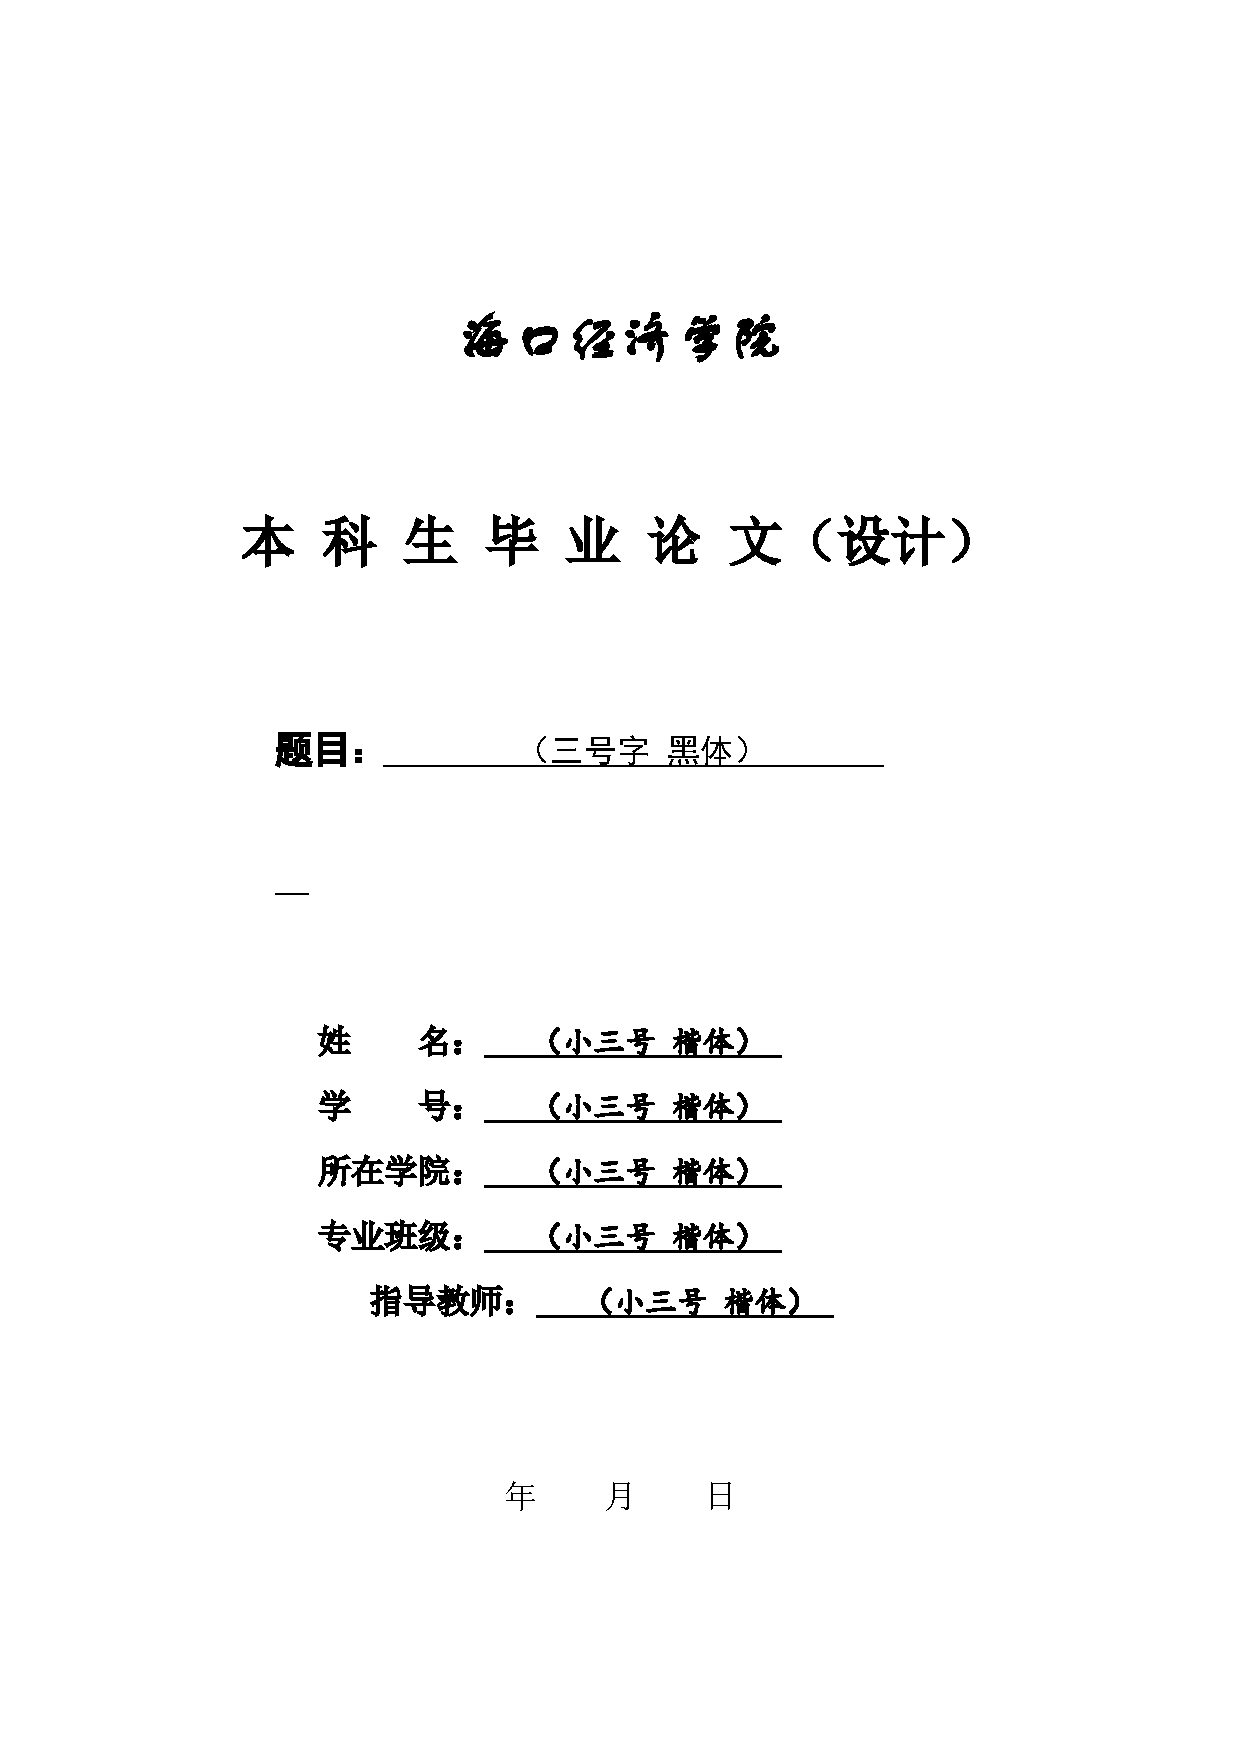
\includepdf[pages={1,2},pagecommand={}]{front.pdf}
\tocpage

\setcounter{page}{1}
\pagenumbering{arabic}

\cnTitleBlock

\cnAbstract{%
  医药行业进入集采常态化与政策严管的深水区后，传统中药龙头正面临需求回撤与战略转型的双重压力。本文以以岭药业为案例，运用趋势分析及杜邦分析法对 2021-2025 年财务报表进行穿透式核查，发现企业因对后疫情需求预测失准产生的“牛鞭效应”，引发了存货积压、资产减值及利润骤降等系统性风险，且由于销售费用等核心成本具有较强的“向下刚性”，在营收缩减期产生了显著的负向经营杠杆。研究表明，企业当前正通过压降营销开支、强化研发强度的“资源配置重心转移”，试图实现由规模扩张向创新驱动的战略变轨，并通过主动出清资产泡沫与优化渠道回款，推动现金流强劲回升。最后，本文建议传统中药企业应推行零基预算管理并构建业财融合的数字化监控系统，以平衡财务稳健性与战略创新，为行业风险防控提供经验借鉴。
}

\cnKeywords{以岭药业；财务风险；资源配置；成本粘性}

\enTitleBlock

\enAbstract{%
  As the pharmaceutical industry enters a "deep-water zone" of normalized volume-based procurement and stringent regulation, traditional TCM leaders face the dual pressures of demand retraction and strategic transformation. This paper takes Yiling Pharmaceutical as a case study, utilizing trend analysis and the DuPont framework to examine its 2021-2025 financial statements, discovering that a "Bullwhip Effect" caused by demand misjudgment led to inventory accumulation, asset impairment, and profit decline, while the "downward rigidity" of costs further squeezed margins during revenue contraction. The analysis shows that the company is currently shifting its resource allocation from marketing to R\&D to transition from scale-driven to innovation-driven growth, achieving a strong cash flow recovery through asset de-bubbling and enhanced channel management. Finally, this paper suggests implementing zero-based budgeting and integrated digital monitoring systems to balance financial stability with strategic innovation, offering risk management insights for the TCM industry.
}

\enKeywords{Yiling Pharmaceutical; financial risk; resource allocation; cost stickiness}

\newpage

\section{引言}
\subsection{研究背景}
以岭药业2025年前三季度的资产减值损失同比增长706.74\%。此现象不是偶然发生的，是中药行业受集采常态化、合规严格管理所造成财务受压的真实反映。由于受院内市场需求的变化影响，企业的存货周转受到很大的阻碍，片剂的库存量激增。库存高企，流动性承压，这已成为企业的核心现状。选择以岭药业作为案例，是因为该企业作为中药行业的头部代表，其核心产品在市场需求波动与政策调整中的表现，具有极强的行业代表性，能够集中反映中药企业在转型期的资产质量变化。

这种业绩变动的深层逻辑在于资源配置的结构性转向。在销售费下降的同时，研发投入仍在提高。资金投向发生转移，实质就是企业缩减营销开支以抵消外部政策压力，在利润空间变小的环境下仍努力保持主要产品的研发投入。尽管 2025年前三季度经营性现金流净额已回归常态水平，但是由于存货跌价和刚性创新投入之间资金的不平衡问题仍然存在。这一调整发生在中药集采全面推行的宏观背景下，研究目的在于探讨企业如何通过调整支出结构来应对利润挤压。其研究意义在于为面临同样政策环境的中药企业提供资源调度的参考方案，防范转型过程中的流动性风险。

\subsection{研究意义}
本研究通过解构以岭药业在政策波动期的资源调度逻辑，旨在探索中药龙头企业实现内生增长回归的具体路径。 在理论层面，本研究通过观察销售费用与研发支出之间的“消长关系”，探讨了企业在营收下滑期如何通过具体科目重组实现风险对冲，弥补了现有文献在药企动态财务调度策略及微观资源配置逻辑研究上的不足。在实践层面，本研究为处于转型期的中药企业提供了可借鉴的财务修复范例：通过计提大额资产减值实现资产质量的去泡沫化，以及通过收紧信用政策将应收账款周转天数由 100.86 天压缩至 60.91 天，展示了企业在极端压力下恢复流动性与增强内源性融资能力的财务手段。研究结论不仅有助于引导中药企业平衡短期盈亏与长期研发投入的关系，实现从营销驱动向创新驱动的战略转型，也为投资者客观评估药企因“科目重组”引发的阶段性亏损提供了决策参考。

\subsection{国内外研究动态}
国外研究动态表明，制药企业财务风险的识别已从单一指标转向多维预警模型与供应链因素的关联性分析。Nugraha 和 Rahadi（2025）通过 Altman Z-Score 模型分析发现，制药行业在后疫情时期呈现出结构性脆弱，微型及小型企业破产风险显著上升，而大型龙头企业则体现出较强的抗风险韧性\textsuperscript{[1]}。Sharma（2023）利用模糊 DEMATEL 方法进一步证实，财务风险与市场需求、物流风险之间存在强关联，且财务压力往往是供应商和运营风险累积后的结果\textsuperscript{[2]}。在风险预警工具上，Feng（2025）针对中国药企改进了 F-score 模型，引入资产现金回报率等指标以提升识别精度\textsuperscript{[3]}。同时，Chudlori（2025）指出企业风险管理（ERM）与公司价值呈正相关，而流动性对价值的影响在特定环境下可能呈现负向特征，凸显了稳健资本结构的重要性\textsuperscript{[4]}。

国内研究动态显示，学术界对财务风险的界定已覆盖企业营运全过程，并针对医药行业的政策敏感性形成了系统性的评价与防范体系。徐焙莹（2023）和张志（2025）明确了广义财务风险涵盖了从筹资、投资到收益分配的全过程，并强调高研发投入虽是核心竞争力，但其不确定性也带来了巨大的投资风险\textsuperscript{[5,6]}。江滢杰（2025）和胡馨雨（2025）指出，资金运营风险潜伏于全过程，具有持续性与隐蔽性\textsuperscript{[7,8]}。在评价方法上，宋星宇和丁桦（2025）与黄冰冰（2025）探讨了从单变量模型向因子分析法、层次分析法（AHP）的演进，以应对政策变动等难以量化的指标\textsuperscript{[9,10]}。针对防范措施，杨玉辉（2025）与张志（2025）主张强化内控环境与现金流管理，树立现金为王的理念\textsuperscript{[6,11]}。黄爱双（2022）则强调，医药集采常态化迫使企业必须从高毛利模式向低成本、规模化及循证医学驱动转型\textsuperscript{[12]}。

国内外研究已在政策敏感性、研发长周期性及现金流稳健性构成的制药企业财务防线方面达成基本共识，但针对大型中药企业在市场剧变下的微观资源调度逻辑仍缺乏深入探讨。 现有文献多侧重于对财务指标的静态评价或行业维度的宏观描述，较少剖析企业如何通过销售支出与研发投入等具体科目的资源重组来应对流动性压力。由于缺乏对企业内部资源配置动态调整过程的研究，难以揭示药企在利润下行周期中实现风险对冲的真实路径。基于此，本文的研究重点转向销售费用与研发支出之间的资源消长关系，旨在通过解构以岭药业的微观科目重组逻辑，弥补现有研究在动态财务调度策略方面的不足，为中药行业平衡生存压力与长期创新投入提供具有操作意义的参考。

\subsection{研究创新与不足}
本文在研究视角的动态性以及对研发资源配置逻辑的重新定义。相比于侧重静态指标的传统财务研究，本文选取了 2022 年至 2025 年这一关键跨度，实时捕捉了以岭药业在市场需求退潮期通过主动缩表实现战略转型的动态全过程。研究创新性地提出了将研发投入作为财务风险对冲工具的逻辑框架，论证了企业如何利用新产品的预期现金流来抵消旧单品受政策挤压导致的毛利损失。此外，本文实现了财务指标与供应链运营风险的深度勾稽，通过将牛鞭效应与 2.48 亿元资产减值损失进行因果关联，提升了财务风险成因分析的穿透力。

受限于案例选择与方法论深度，本研究在普遍适用性及量化精度方面仍存在一定不足。 由于本研究以以岭药业为单一分析对象，所得出的“销转研”对冲逻辑在中小规模药企及其他细分领域的普适性仍有待进一步验证。在分析方法上，本文主要采用趋势分析及对比分析等描述性研究手段，缺乏利用计量经济学模型对各项风险因子贡献度进行精确测算，这在一定程度上限制了风险预警逻辑的实证精度。

\section{相关概念与理论基础}
\subsection{医药行业财务特征}
医药行业的财务表现深受宏观政策与行业特性的交织影响，呈现出显著的结构性脆弱。集采政策（VBP）的常态化推行正迫使企业从传统的高毛利、重营销模式向低成本及循证医学驱动转型，黄爱双 (2022) 强调价格的阶梯式下行挤压了利润空间，使得过往依赖高销售费用驱动的增长模式引发了严重的费用粘性与利润反噬冲突。此外，医药制造业高研发、高不确定性的特点，导致大规模投入在短期内可能使资本效率降至零点，徐焙莹 (2023) 指出这种研发强度的加法与营收放缓的减法之间的博弈，构成了企业财务结构中最为核心的风险变量。

从中药行业特定的生产属性来看，对原材料种植、季节性采收及前置储备的高度依赖进一步放大了供应链的波动风险。Sharma (2023) 认为财务风险与需求及物流风险具有强因果关系，直接诱发了运营及供应商风险。结合中药生产特性，刘倩倩 (2025) 发现当企业面对爆发性需求而盲目扩大排产时，极易诱发牛鞭效应，这种生产端对终端需求的过度反馈会导致存货积压并形成资金堰塞湖。这一机理不仅解释了中药企业在需求回撤期的流动性挤压逻辑，更揭示了资产质量劣化与财务稳健性受损的深层诱因。

\subsection{相关概念}
\subsubsection{财务风险定义}
财务风险的界定已由单一融资风险演变为涵盖筹资、投资、运营及收益分配的广义风险观，其本质是资源配置效率与外部市场波动间的逻辑冲突。从机理上看，风险不仅体现为流动性断裂，更反映在资产价值贬损与资本结构失衡上；当经营决策、财务控制与政策调整、行业竞争步调失准时，价值链任何环节的失控均会引发指标异常。从动态属性分析，风险具有显著的传导性与滞后性，往往发端于业务端的需求错配或费用扩张，通过营运周转减速渗透至利润表，最终沉淀于资产负债表并削弱内源性融资能力。在战略视角下，财务风险是转型成本与财务承受力的博弈，尤其在医药行业，表现为研发长期性与回报不确定性的错位，以及转型期费用粘性对利润的压榨。综上，财务风险是企业在追逐价值增值时，因资源配置不当、环境响应迟滞或战略偏离，导致财务状况恶化及生存边界受损的不确定状态。

\subsubsection{财务风险分类}
财务风险作为企业经营不确定性的集中体现，贯穿于资金循环的全过程。结合医药制造业高研发投入、高销售费用及政策高度敏感的行业属性，本文将财务风险划分为偿债能力、营运能力、盈利能力及发展能力四个维度进行系统界定。偿债能力风险聚焦于资本结构与现金流稳定性，反映企业履行到期债务的安全性；营运能力风险侧重于资产配置效率，核心关注在“牛鞭效应”影响下存货与应收账款的周转水平；盈利能力风险体现为受集采政策与“费用粘性”挤压时利润空间的稳健性；最后，发展能力风险则指向企业的战略成长性，重点考察研发驱动下的品种迭代与市场扩张潜力。这四个维度构成了本文后续对以岭药业进行财务风险识别与穿透式分析的核心理论框架。

\subsubsection{财务风险评价方法}
财务风险评价体系正由单一财务指标分析向“模型改进、系统风控与战略决策”的综合框架转型。 在定量预警方面，宋星宇和丁桦（2025）与 Nugraha 和 Rahadi（2025）均强调了Altman Z-Score 模型在预测企业破产风险中的普遍适用性\textsuperscript{[1,9]}；而 Feng和Feng（2025）针对中国制药企业改进了 F-score 模型，引入“资产现金回报率”以提升识别精度\textsuperscript{[3]}。为克服主观偏差，黄冰冰（2025）提出利用因子分析法进行降维处理，使评价结果更具客观性\textsuperscript{[10]}。此外，苏川（2025）与胡馨雨（2025）主张将层次分析法（AHP）与智能决策支持系统相结合，利用大数据关联分析找出业务活动中的隐性成本，为动态识别资源错配赋予了技术手段\textsuperscript{[8,13]}。

财务风险评价体系正由单一指标分析向模型改进、系统风控与战略决策的综合框架转型。在定量预警方面，学者们通过 Altman Z-Score 模型、改进的 F-score 模型以及因子分析法，不断提升对破产风险与识别精度的客观判定。此外，层次分析法（AHP）与大数据关联分析的结合，也为动态识别业务活动中的隐性成本提供了技术支撑。然而，定量模型虽能通过历史数据测算财务危机的概率，却难以分析行业政策变动时的风险，难以实现对风险生成机理的深度还原，因此，本文选用案例分析法作为主要研究手段，通过对以岭药业这一典型样本的深度剖析，本文旨在从业务机理、战略以及管理对策三个维度，构建起从经营本质到财务结果的完整逻辑闭环，从而为同类企业提供更具操作性的风险对冲模型与财务防御建议。

\subsection{理论基础}
\subsubsection{牛鞭效应理论}
牛鞭效应描述了供应链上需求信息由下游向上传递时，由于信息扭曲与反馈时滞，导致波动逐级放大的现象。该理论最早由 Forrester (1961) 提出，后经 Lee 等 (1997) 系统化，指出需求预测修正、订货批量决策、价格波动以及短缺博弈是诱发波动的核心变量。当终端市场需求发生微小变动时，零售商、批发商及生产商基于各自的预测逻辑，会层层放大订单量或库存储备。这种现象会导致生产端的排产计划严重脱离真实市场需求，最终使企业在下行周期中积压大量营运资金。这种产需错配的本质，是供应链响应机制与外部政策及市场环境变动之间的逻辑冲突。本文利用该理论解释以岭药业在呼吸系统类产品需求波动中的产需错配风险。通过分析管理层如何将短期爆发性需求误判为长周期增长趋势，进而层层放大生产排产与物料储备，揭示其导致存货积压、营运资金占用及后续资产大额减值的财务逻辑。

\subsubsection{费用粘性理论}
费用粘性理论是指企业成本变动与业务量变动之间存在的不对称性，即业务量下降时的费用减幅小于业务量等比例上升时的费用增幅。Anderson 等 (2003) 通过实证研究确认了这一现象，挑战了传统管理会计中成本与业务量线性关系的假设。其核心诱因包括资源调整成本、管理层心理预期及长期契约约束。该理论应用于分析以岭药业在营收阶梯式回落期利润受损的深层原因。重点探讨重资产营销模式下，人员安置、渠道维护等刚性支出如何产生调整滞后，进而通过经营杠杆效应产生利润反噬，以此评估企业费用结构对财务韧性的影响。

\section{以岭药业概况}
\subsection{以岭药业概况}
石家庄以岭药业股份有限公司（以下简称以岭药业）由中国工程院院士吴以岭于 1992 年创立，总部位于河北石家庄。经过三十余年的发展，公司已成长为一家集研发、生产和销售于一体的中国医药行业头部上市企业。在行业地位方面，以岭药业位居中国中药企业前十强，并多次入选中国品牌价值百强榜单，是国内衡量创新驱动型中药企业的标杆。

\subsection{主营业务}
以岭药业作为国内中药创新药的领军企业，其主营业务高度集中于专利中药的研发、生产与销售。公司依托络病证治理论体系，构建了多元化的产品矩阵，核心业务主要由呼吸系统类产品、心脑血管类产品、二线及新兴品种板块三大板块构成，其中，呼吸系统类产品以连花清瘟系列为代表，该板块在公司总营收中占据主导地位。在特殊需求周期内，其收入占比曾一度超过50\%，是公司现金流的主要来源。然而，随着市场需求回归常态及集采政策的推进，该板块正面临从“爆发式增长”向“稳健存量市场”的结构性调整；心脑血管类产品主要包括通心络胶囊、参松养心胶囊及芪苈强心胶囊等专利品种。该板块市场准入壁垒较高，具有较强的客户黏性和长期复购特征，在公司收入结构中发挥着“稳压器”作用，其毛利率水平持续保持在行业领先地位；二线及新兴品种涵盖了糖尿病药（津力达颗粒）、抗衰老（八子补肾胶囊）及化药等领域。公司近年通过“科目位移”策略，将更多资源向该领域倾斜，旨在通过品种多元化分散对单一口服抗病毒产品的过度依赖，优化整体收入结构。

以岭药业财务表现从早期的快速规模扩张转入到资产重组与内源性融资能力重建的深度调整期，完整展示了大型药企在市场红利消退后，如何通过会计科目位移与营运资本政策调整来应对流动性风险的典型逻辑。因此，选取以岭药业进行案例分析，对于探讨中药企业如何在外部强干扰下平衡研发投入与财务稳健性具有重要的学术参考价值。

\section{财务风险识别}
\subsection{偿债风险识别}
偿债能力反映企业偿还债务的能力，分为短期偿债能力和长期偿债能力两类。短期偿债分析旨在评估企业对即期债务的响应速度。通过流动比率考察整体变现能力，利用速动比率剔除变现较慢的存货以评估极端情况下的偿付力，并结合货币资金余额直接观测企业的现金储备厚度，从而全面识别经营波动对资金链的实时压迫。长期偿债分析侧重于评估企业的资本结构稳健性与财务杠杆风险。通过资产负债率衡量企业对外部债权人资金的依赖程度，利用产权比率揭示自有资金与债务资金的配比关系（即财务杠杆），从而识别企业在长期经营周期内抵御行业波动的财务韧性。

\subsubsection{短期偿债风险识别}
\paragraph*{流动比率}
从表4-1可以看出，流动比率方面，2021—2025年分别为1.89、1.50、1.47、1.66和2.36，总体呈先降后升态势，各年均高于公认安全线1.0。但2022—2023年流动比率明显下滑（由1.89降至1.47），表明连花清瘟疫情红利消退后短期偿债压力有所上升，2025年大幅回升至2.36，流动性状况显著改善。

\paragraph*{速动比率}
2021—2025年的速动比率分别为1.33、1.08、0.92、0.99和1.68，2023年首次跌破1.0，降至0.92，说明扣除存货后流动资产已不足以覆盖全部流动负债，短期流动性存在一定压力；2025年大幅回升至1.68，流动性紧张局面显著缓解。

\paragraph*{货币资金}
货币资金方面，2022年大幅增加至19.04亿元，与连花清瘟销售爆发直接相关；2023年骤降至9.41亿元，2024年进一步降至8.53亿元，显示企业现金储备压力加大；2025年回升至11.05亿元，现金状况有所改善。

\begin{thesTab}[htbp]{短期偿债分析指标\label{tab:t1}}{}
\begin{tabularx}{\linewidth}{X c c c c c}
  \toprule
  指标 & 2021年 & 2022年 & 2023年 & 2024年 & 2025年 \\
  \midrule
  流动资产（亿元） & 56.02 & 72.54 & 65.44 & 43.35 & 52.06 \\
  流动负债（亿元） & 29.6 & 48.5 & 44.47 & 26.07 & 22.08 \\
  货币资金（亿元） & 9.95 & 19.04 & 9.41 & 8.53 & 11.05 \\
  流动比率 & 1.89 & 1.5 & 1.47 & 1.66 & 2.36 \\
  速动比率 & 1.33 & 1.08 & 0.92 & 0.99 & 1.68 \\
  \bottomrule
\end{tabularx}
\end{thesTab}

\begin{figure}[htbp]
  \centering
  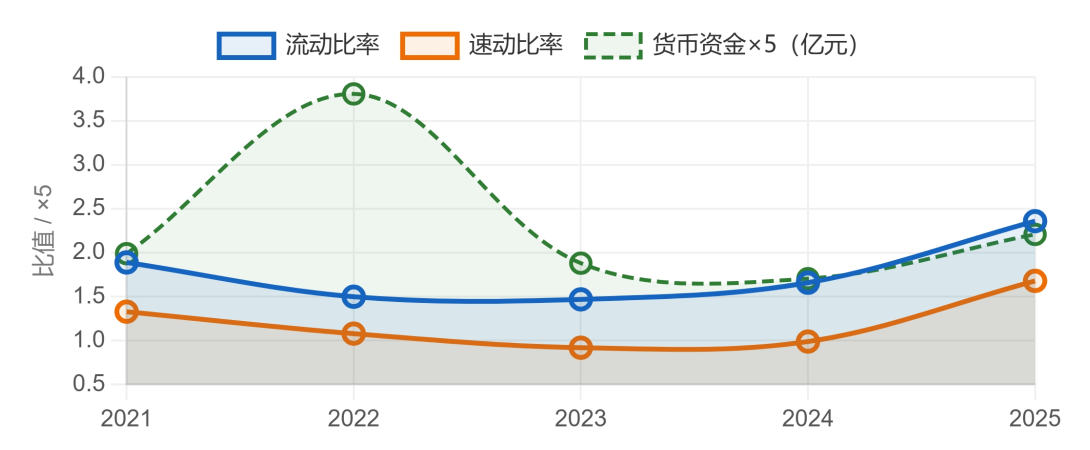
\includegraphics[width=0.82\linewidth]{figures/fig1.png}
  \caption{短期偿债分析指标图}\label{fig:f1}
\end{figure}

\subsubsection{长期偿债风险识别}
从表4-2来看，以岭药业整体资产负债率偏低，远低于医药制造业平均水平（约40\%～50\%），说明企业长期偿债能力较强，财务结构较为稳健。2022年资产负债率跳升至29.69\%，主要受连花清瘟爆发期扩大生产规模、增加短期借款所致。2024年大幅下降至19.57\%，2025年进一步降至16.15\%，反映出企业主动压缩负债的审慎态度。产权比率各年均在0.20～0.44之间，整体较低，表明企业以股权融资为主，长期偿债风险相对可控。

\begin{thesTab}[htbp]{长期偿债能力指标\label{tab:t2}}{数据来源：以岭药业2021-2025年年度报告}
\begin{tabularx}{\linewidth}{X c c c c c}
  \toprule
  指标 & 2021年 & 2022年 & 2023年 & 2024年 & 2025年 \\
  \midrule
  总资产（亿元） & 129.05 & 163.36 & 169.79 & 133.19 & 136.75 \\
  总负债（亿元） & 29.6 & 48.5 & 44.47 & 26.07 & 22.08 \\
  归母净资产（亿元） & 90.69 & 109.32 & 114.5 & 102.23 & 109.89 \\
  资产负债率 & 22.94\% & 29.69\% & 26.19\% & 19.57\% & 16.15\% \\
  产权比率 & 0.33 & 0.44 & 0.39 & 0.26 & 0.2 \\
  \bottomrule
\end{tabularx}
\end{thesTab}

\begin{figure}[htbp]
  \centering
  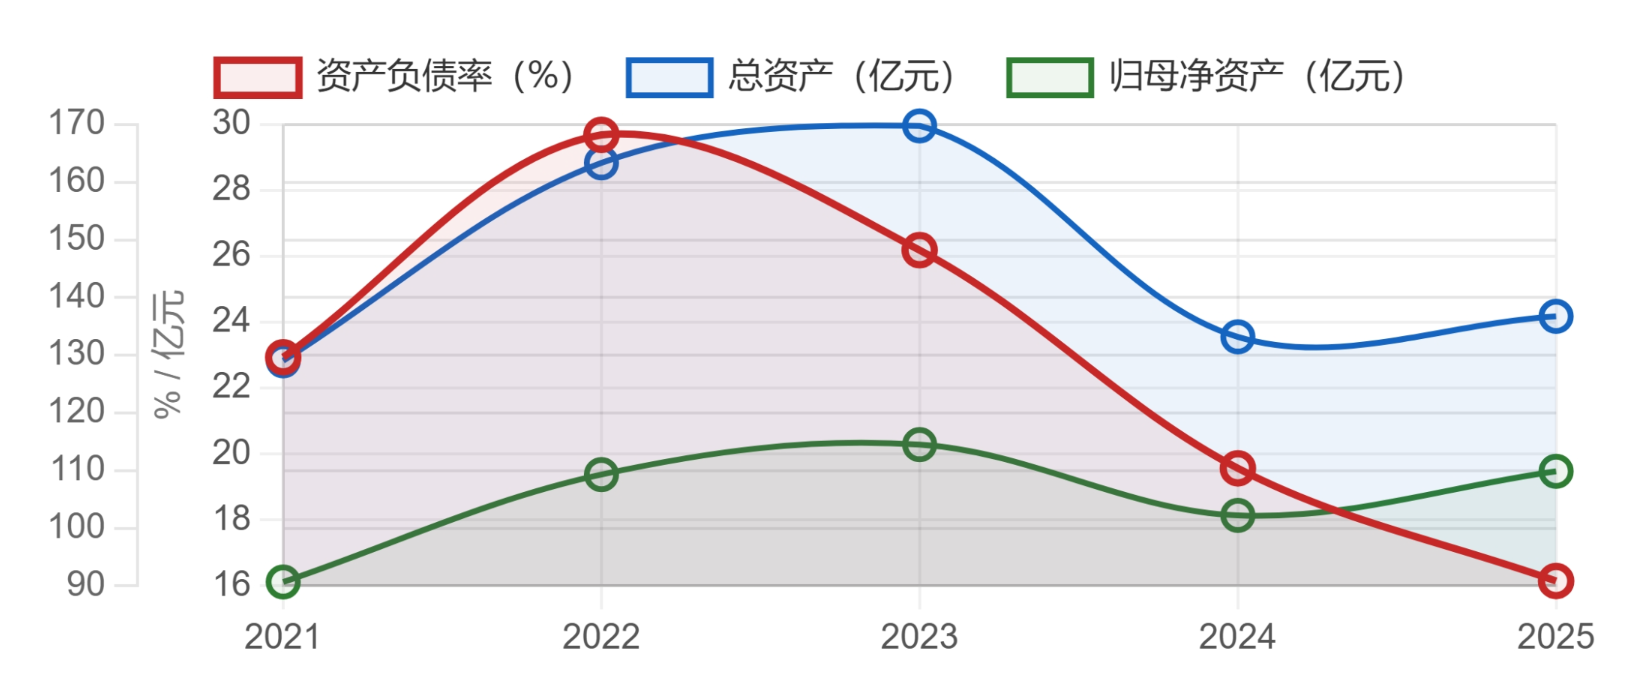
\includegraphics[width=0.82\linewidth]{figures/fig2.png}
  \caption{长期偿债能力分析图}\label{fig:f2}
\end{figure}

以岭药业目前的偿债风险呈现出底蕴深厚但局部紧绷的特征。公司财务结构极度稳健，资产负债率常年处于 20\% 以下的行业极低水平，长期偿债能力具备极强的战略防御力。2023 至 2024 年间，货币资金从峰值骤降超过 50\%，且速动比率一度跌破 1.0 的安全线，这揭示了在营收失速背景下，企业现金流缓冲垫正在收窄。这种静态资产雄厚、动态现金承压的矛盾，暴露出企业对突发政策或市场波动的调节灵活性不足。

\subsection{营运风险识别}
营运能力分析的核心在于识别资产周转过程中的资金沉淀风险。通过应收账款周转率与存货周转率评估经营活动中现金回笼的速度与效率，结合总资产周转率考察全盘资产的利用水平，从而揭示营收规模收缩时可能出现的资源闲置与坏账风险。具体数据如表4-3所示。

\paragraph*{应收账款周转率}
2021—2022年分别为6.28次和7.26次，收款效率处于较高水平；2023年大幅下降至4.30次，为五年最低，表明疫情期间连花清瘟虽然销量爆发，但回款情况并不理想，应收账款积压明显。2024年应收账款周转率回升至5.31次，2025年进一步升至6.37次，得益于公司加大回款催收力度和应收账款绝对额的减少（由24.01亿元降至12.29亿元）。但整体来看，2023年应收账款高达24.01亿元，较2021年增长49.1\%，存在较大的坏账风险。

\paragraph*{存货周转率}
2022年存货周转率为6.20次，较为健康；但2023年降至4.20次，2024年进一步降至3.73次，呈持续恶化趋势。这与疫情期间大规模扩产、疫情结束后需求骤降导致的库存积压直接相关。2025年存货周转率显著反弹至5.26次，库存管理效率明显改善。

\paragraph*{总资产周转率}
2021—2022年分别为0.78次和0.77次，资产利用效率较为稳定；2023年降至0.61次，2024年进一步降至0.49次，资产效率持续下滑，说明企业在疫情红利消退后，资产结构调整滞后，存量资产未能得到充分利用。2025年总资产周转率回升至0.57次，显示资产运营效率有所改善但尚未恢复至疫情前水平。

\begin{thesTab}[htbp]{营运风险分析指标\label{tab:t3}}{数据来源：以岭药业2021-2025年年度报告}
\begin{tabularx}{\linewidth}{X c c c c c}
  \toprule
  指标 & 2021年 & 2022年 & 2023年 & 2024年 & 2025年 \\
  \midrule
  营业收入 & 101.17 & 125.33 & 103.18 & 65.13 & 78.31 \\
  应收账款 & 16.11 & 17.27 & 24.01 & 12.25 & 12.29 \\
  存货 & 16.73 & 20.22 & 24.59 & 17.46 & 14.89 \\
  应收账款周转率（次） & 6.28 & 7.26 & 4.3 & 5.31 & 6.37 \\
  存货周转率（次） & 6.05 & 6.2 & 4.2 & 3.73 & 5.26 \\
  总资产周转率（次） & 0.78 & 0.77 & 0.61 & 0.49 & 0.57 \\
  \bottomrule
\end{tabularx}
\end{thesTab}

\begin{figure}[htbp]
  \centering
  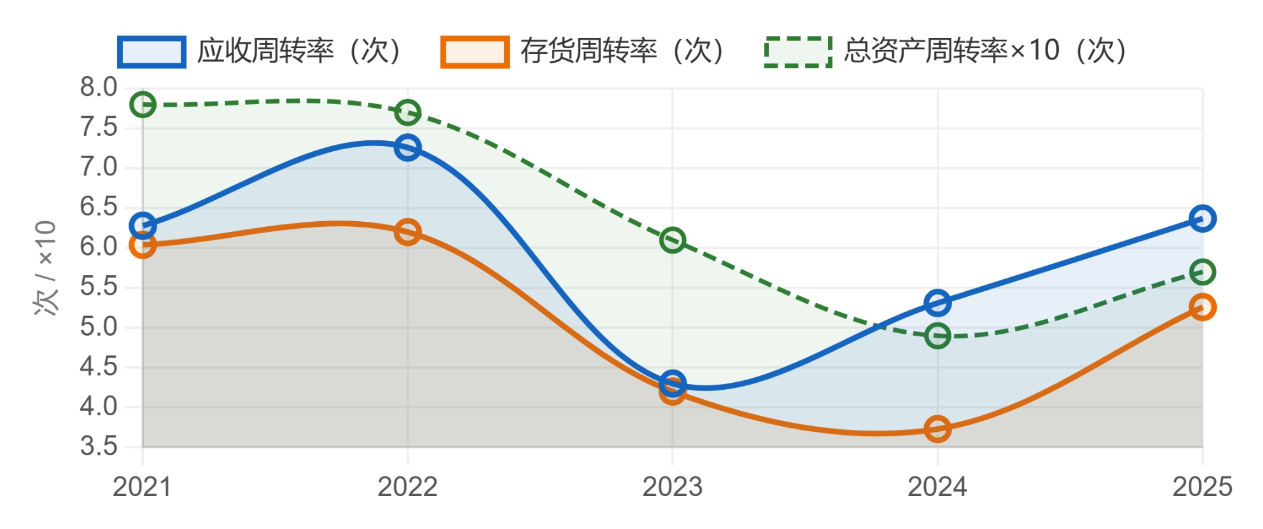
\includegraphics[width=0.82\linewidth]{figures/fig3.png}
  \caption{营运风险分析图}\label{fig:f3}
\end{figure}

以岭药业的营运风险呈现出核心资产周转回暖，但整体资源配置冗余的特征。2025 年公司通过强化回款和去库存，有效盘活了应收账款与存货，缓解了经营性资金占用；但总资产周转率仍处于历史低位，反映出在营收规模收缩后，庞大的存量资产（厂房、设备等）调整明显滞后，形成了结构性闲置。这种局部好转而整体低效的状态，意味着企业仍面临较高的资产维护成本与资源浪费风险，亟需在未来通过资产剥离或产能优化来提升全盘经营效能。

\subsection{盈利风险识别}
盈利能力分析旨在评估企业利润生成的效率与股东回报的稳定性。盈利能力是企业可持续发展的根本动力，盈利能力下降是财务风险最直观的信号。通过 净资产收益率（ROE）衡量自有资本的增值效率；利用总资产净利率（ROA）考察全盘资产（含债务）的管理效能，以识别重资产配置与营收规模的匹配度；结合 每股收益（EPS）直观反映投资者回报的波动性。通过多指标对比，能够深度识别企业在业绩起伏中是否存在虚假繁荣或防御性收缩等结构性风险，具体如表4-4所示。

\paragraph*{总资产净利率（ROA）}
总资产净利率（ROA）衡量的是企业利用全部资产（包括自有资金和债务）获取利润的能力。以岭药业的 ROA 从 2022 年的 14.46\% 断崖式下跌至 2024 年的 -5.44\%，这表明在营收缩减时期，企业的固定资产、存货等重资产配置未能及时调整，导致资产负担过重。虽然 2025 年 ROA 回升至 9.37\%，但仍未触及 2021 年水平。

\paragraph*{加权平均 ROE}
从表3.3中数据可见，以岭药业的 ROE 经历了个极端的过山车式波动。从 2022 年 23.62\% 的历史巅峰，骤降至 2024 年的 -6.69\%。这种大幅转负意味着股东投入的资本不仅没有产生增值，反而处于缩水状态。尽管 2025 年 ROE 回升至 11.99\%，但尚未恢复到 2021 年 14.94\% 的常态水平，这反映出企业自有资本的获利效率在外部冲击后仍处于脆弱的修复期。

\paragraph*{每股收益（EPS（元）}
EPS 直接关系到投资者的持股收益。2022 年 1.41 元的超额回报是由特殊需求拉动的，而 2024 年的 -0.43 元则是上市以来的首次严重“负回报”。这种剧烈的波动性向市场传递了极其不稳定的信号，极大地增加了二级市场的股价波动风险和企业融资成本。2025 年 EPS 虽然修复至 0.77 元，几乎追平 2021 年。但需要识别的是，这种修复背景是 2025 年营收规模（78.31亿）远小于 2021 年（101.17亿）。这种“低营收、高EPS”的异动，反映出企业在 2025 年进行了强力且不可持续的成本压缩（如削减销售费用或管理费用），若未来收入无法重回百亿大关，EPS 的长期稳定性依然存疑。

\begin{thesTab}[htbp]{盈利风险分析指标\label{tab:t4}}{数据来源：以岭药业2021-2025年年度报告}
\begin{tabularx}{\linewidth}{X c c c c c}
  \toprule
  指标 & 2021年 & 2022年 & 2023年 & 2024年 & 2025年 \\
  \midrule
  营业收入（亿元） & 101.17 & 125.33 & 103.18 & 65.13 & 78.31 \\
  归母净利润（亿元） & 13.44 & 23.62 & 13.52 & -7.25 & 12.86 \\
  营业利润率 & 15.51\% & 22.58\% & 17.25\% & -10.58\% & 20.73\% \\
  加权平均ROE & 14.94\% & 23.62\% & 12.16\% & -6.69\% & 11.99\% \\
  总资产净利率（ROA） & 10.40\% & 14.46\% & 7.97\% & -5.44\% & 9.37\% \\
  每股收益（EPS（元） & 0.8 & 1.41 & 0.81 & -0.43 & 0.77 \\
  \bottomrule
\end{tabularx}
\end{thesTab}

\begin{figure}[htbp]
  \centering
  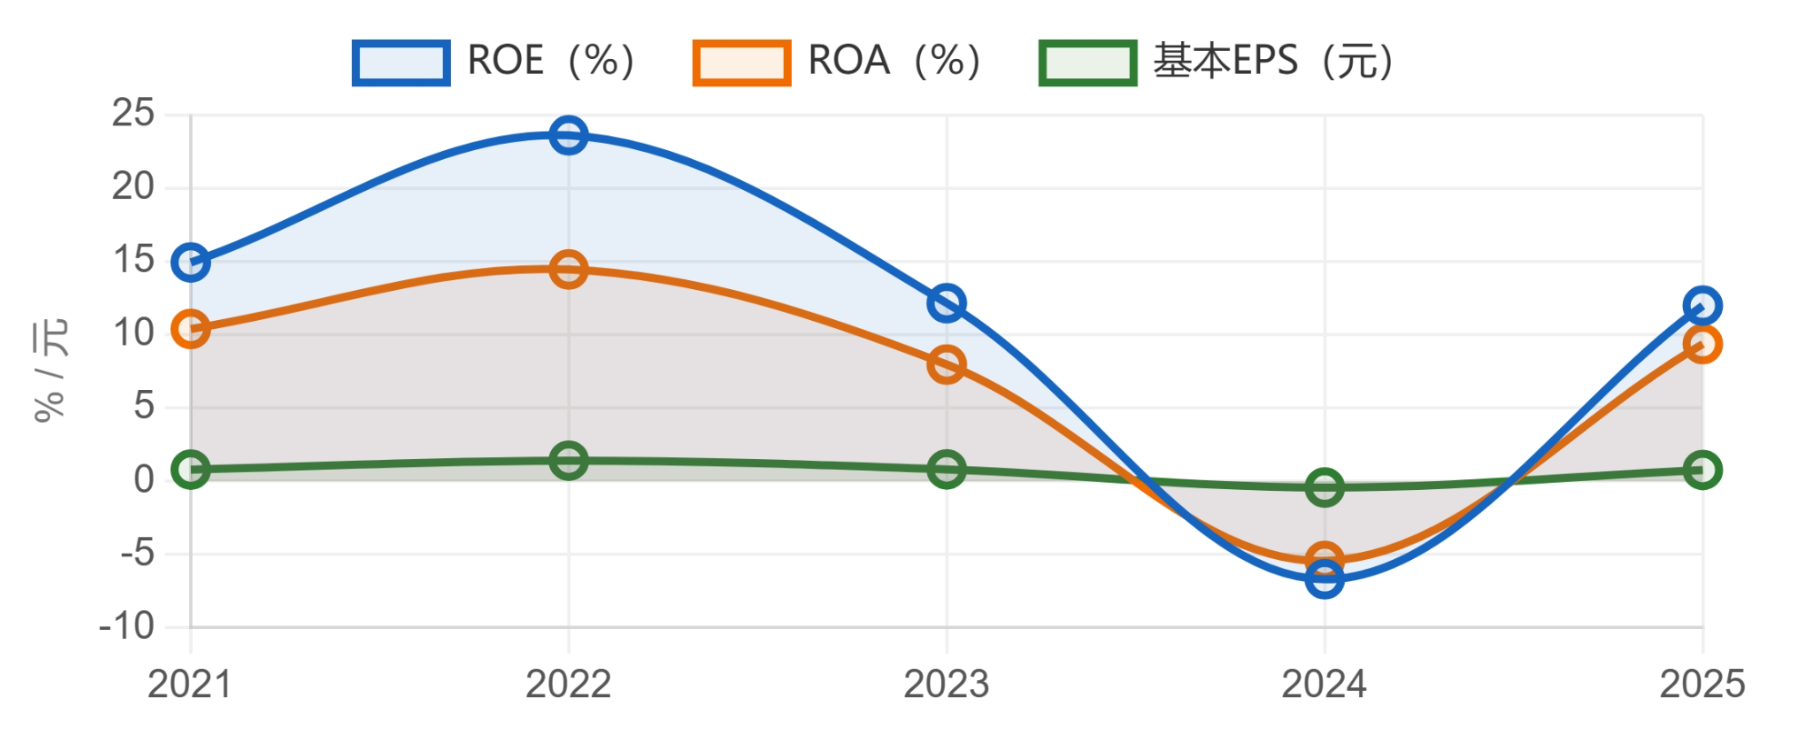
\includegraphics[width=0.82\linewidth]{figures/fig4.png}
  \caption{营运风险分析图}\label{fig:f4}
\end{figure}

以岭药业的盈利能力呈现出剧烈波动及复苏脆弱的特征。其 ROA 从 2022 年的高点断崖式转负，暴露了营收萎缩下重资产配置过载的风险；EPS 的极端震荡则严重损害了股东回报的稳定性。尽管 2025 年利润有所回升，但在营收规模远不及往年的背景下，这种依靠成本压缩实现的“低营收、高收益”现象，反映出企业增长后劲不足，盈利的可持续性依然面临严峻挑战。

\subsection{发展风险识别}
发展能力分析旨在识别企业增长的稳定性与利润的真实变现力。通过营业收入增长率与净利润增长率的对比，观测企业是否存在对单一品种的过度依赖及业绩波动的极端性；结合经营活动现金流量净额与净利润的勾稽关系，识别账面利润的含金量，从而揭示企业在规模扩张过程中是否存在“虚盈实亏”或现金流断裂的潜在风险，具体数据如表4-5所示。

营业收入增长率

以岭药业营收增长率在五年内经历了大幅波动。2021年增长20.15\%，2022年增长23.90\%至125.33亿元峰值，2023年急转直下降17.67\%至103.18亿元，2024年暴跌36.89\%至65.13亿元，2025年强劲反弹20.24\%至78.31亿元。超高的营收波动性说明公司收入高度依赖连花清瘟这一单一品种，收入结构风险极为显著。

净利润增长率

2022年净利润增长75.75\%，2023年下降42.72\%，2024年骤降153.58\%（由盈转亏），2025年反弹277.39\%至12.86亿元。净利润的超高波动性是以岭药业核心的财务风险特征，折射出核心产品周期性极强、抗风险能力薄弱的深层问题。

总资产增长率和净资产增长率

总资产与净资产先扩后缩。2022年总资产增长26.59\%至163.36亿元，为五年峰值；2024年总资产大幅缩减21.53\%至133.19亿元，是企业主动收缩规模、消化库存的体现。2025年总资产小幅回升至136.75亿元（+2.67\%），净资产增长7.49\%至109.89亿元，资产规模基本企稳。

\begin{thesTab}[htbp]{发展能力风险及现金流汇总表\label{tab:t5}}{数据来源：以岭药业2021-2025年年度报告}
\begin{tabularx}{\linewidth}{X c c c c c}
  \toprule
  指标 & 2021年 & 2022年 & 2023年 & 2024年 & 2025年 \\
  \midrule
  营业收入增长率 & 15.19\% & 23.88\% & -17.67\% & -36.88\% & 20.24\% \\
  净利润增长率 & 10.27\% & 75.75\% & -42.76\% & -153.57\% & 277.56\% \\
  总资产增长率 & 12.29\% & 26.59\% & 3.91\% & -21.56\% & 2.67\% \\
  净资产增长率 & 1.68\% & 20.54\% & 4.73\% & -10.71\% & 7.49\% \\
  经营活动现金流量净额 & 5.29 & 34.88 & 1.55 & 6.11 & 17.77 \\
  \bottomrule
\end{tabularx}
\end{thesTab}

\begin{figure}[htbp]
  \centering
  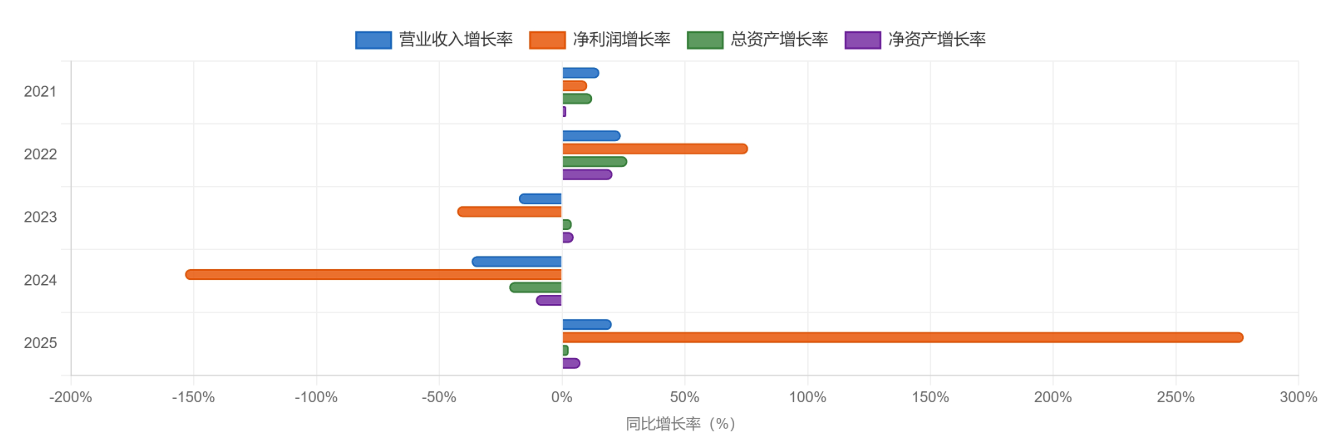
\includegraphics[width=0.82\linewidth]{figures/fig5.png}
  \caption{发展能力风险分析图}\label{fig:f5}
\end{figure}

\paragraph*{经营活动现金流量}
经营现金流波动剧烈且与净利润严重背离。2022年经营活动现金流净额高达34.88亿元，远超当年净利润23.62亿元，说明该年度不仅盈利丰厚，而且回款质量极高；但2023年经营现金流骤降至1.55亿元，较2022年剧降95.55\%，而当年净利润仍有13.52亿元，两者严重背离，表明账面利润质量存疑，存在大量应收账款未能及时回笼。2024年经营现金流回升至6.11亿元，2025年进一步改善至17.77亿元，现金流质量显著提升。

\begin{figure}[htbp]
  \centering
  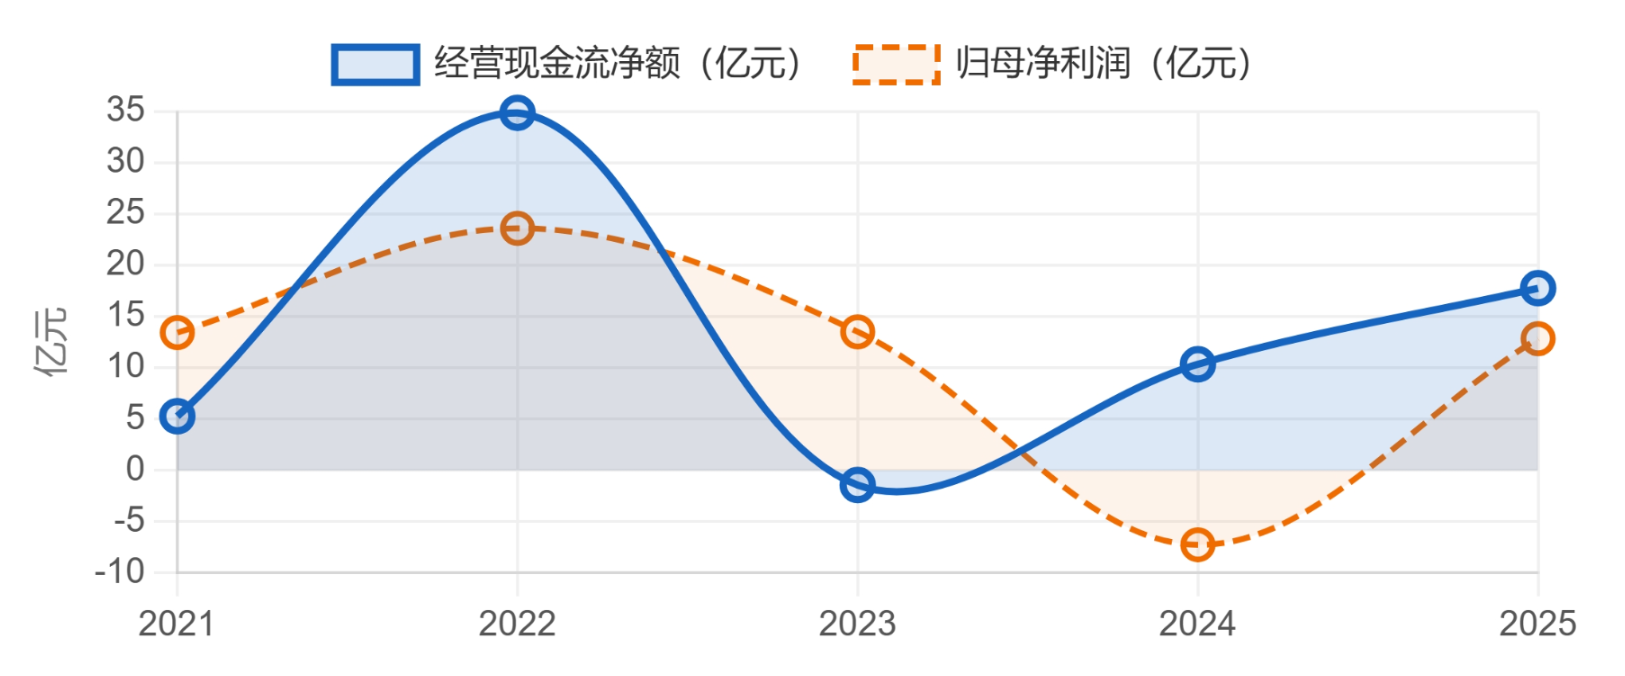
\includegraphics[width=0.82\linewidth]{figures/fig6.png}
  \caption{现金流与归母净利润分析图}\label{fig:f6}
\end{figure}

以岭药业在发展维度上呈现出爆发力强但稳定性缺失，现金回流滞后于利润确认的特征。公司在市场机遇期具备极强的业绩爆发力，且 2025 年的现金流修复说明其具备较快的自我纠偏能力。超高波动的业绩曲线揭示了企业严重缺乏对冲行业震荡的第二增长”，且经营现金流与利润的频繁脱节，暴露出收入结构中隐含的变现风险。这种“脉冲式”增长模式不仅增加了经营预测难度，更为企业未来的持续性研发投入与股利分配带来了极大的不确定性，是后续成因分析中需重点关注的战略软肋。

\section{以岭药业财务风险成因分析}
针对前节识别出的以岭药业在偿债、盈利、营运及发展能力四个维度的财务风险点特别是 2024 年的历史性亏损与 2025 年的节流型复苏，本节将结合医药行业特征，深度穿透剖析其风险形成的深层逻辑。

\subsection{偿债能力成因分析}
企业的偿债能力不仅取决于资产规模，更取决于现金流的产生与转化效率。当企业为了维持账面营收而采取激进的信用政策（如放宽回款期限）时，会导致现金转化周期拉长，出现账面繁荣而现金枯竭的流动性危机。以岭药业在2023年至2024年间短期偿债压力骤增，速动比率一度跌至0.92的危险水平。其深层原因在于管理层在后疫情需求回落期，为保住市场份额，对下游经销商采取了 “回款换销量”的策略。应收账款周转天数从2022年的约35天猛增至2024年的100.86天。这种回款效率的断崖式下跌，导致2023年经营性现金流仅为1.55亿元，净现比低至0.11，迫使企业频繁动用募集资金补充流动性，严重削弱了动态偿债保障。

\subsection{营运能力风险成因分析}
营运能力风险的累积是前期激进扩张策略与后期需求萎缩叠加作用的必然结果。库存管理失控方面，疫情期间盲目扩大产能，存货规模从2021年的16.73亿元攀升至2023年的24.59亿元，存货周转率却从6.04次持续下降至3.73次，2024年被迫计提减值准备直接侵蚀利润超过16亿元。应收账款管理不力方面，2023年应收账款高达24.01亿元，较2021年增长49.1\%，远超同期营收增长率，表明公司在追求销售规模的同时放松了信用管理，销售回款周期明显拉长。总资产周转率的持续下降（由0.78次降至0.49次）则反映出大量专用生产线在疫情红利消退后处于闲置或低负荷运转状态，固定成本负担加重，资产运营效率系统性下滑。

\subsection{盈利能力风险成因分析}
以岭药业的盈利能力受费用结构的柔性及对核心产品毛利空间的动态管控能力影响。在医药行业中，集采导致的价格下行与原料上涨发生冲突时，以岭药业将面临盈利塌陷的系统性风险。以岭药业的心血管系列芪苈强心胶囊、通心络胶囊等产品均面临纳入集采或区域联盟采购的压力，价格下行直接压缩毛利率空间，另一方面上游原材料（如酸枣仁）价格暴涨，导致呼吸系统类产品毛利率从 69.19\% 剧烈滑坡至 42.97\%。

同时，研发投发增长和销售费用难以下降也进一步冲击以岭药业盈利空间。从财务数据看，营收虽缩减近 37\%，但具有费项粘性的销售费用仅小幅下调，导致销售费用率逆势飙升，产生剧烈的经营杠杆负效应；同时，企业在利润失速期仍坚持高强度的研发投入（强度达 13.94\%），虽构建了长期护城河，但在新药贡献业绩前形成了巨大的产出时滞与盈利真空。这种成本缩减的滞后性与跨周期研发投入的刚性重叠，迅速耗尽了企业的毛利缓冲空间，直接导致了当年的深度亏损。

\subsection{发展能力风险成因分析}
发展能力风险的本质是企业在外部环境剧烈变化背景下战略调整滞后与内生增长动力不足的集中体现。以岭药业2021—2025年营收的剧烈波动几乎完全由疫情周期所驱动，而非源于产品竞争力提升或市场开拓进展。公司在心脑血管、糖尿病、肿瘤等具有长期增长潜力的治疗领域的拓展进展缓慢，新产品上市节奏不足以弥补连花清瘟需求下降留下的收入缺口，2025年上半年营收已连续7个季度录得同比负增长。2023年经营现金流骤降至1.55亿元而净利润仍有13.52亿元，两者巨大落差说明盈利质量存在严重问题——大量销售仅形成账面收入而未实际回款，资金被库存所占用。2024年总资产较2022年峰值减少30.17亿元（降幅达18.5\%），这并非源于理性的资产结构调整，而是疫情红利消退后被迫消化前期过度扩张的代价，资产规模的收缩不仅削弱了经营实力，也向资本市场传递了负面信号。

\section{以岭药业财务风险防范对策}
\subsection{偿债能力风险防范对策}
\paragraph*{建立流动性风险预警机制，设置多层级安全线。}
以岭药业应参照医药行业特性，建立适合自身的流动性风险管理框架。建议设定三档预警阈值：流动比率低于1.5时发布黄色预警，低于1.2时发布橙色预警，低于1.0时启动紧急流动性干预。同时，将货币资金保有量与刚性债务偿还需求挂钩，确保货币资金不低于未来6个月到期债务本息之和的1.5倍，形成充足的安全垫。

\paragraph*{优化债务期限结构，化解集中到期风险。}
公司应根据项目周期和现金流匹配原则，将部分短期借款置换为中长期债务，降低短期债务集中到期的偿付压力。建议将短期借款占总借款比重控制在40\%以内，并建立债务到期管理台账，提前6个月制定再融资方案，避免被动展期或违约风险。

建立集中资金管理平台，强化现金统筹调配。

建议建立集团级资金集中管理平台，实现对子公司资金的统一归集与调配，提高闲置资金使用效率。同时建立现金流量预测模型，滚动预测未来3—6个月的现金收支缺口，提前采取融资或收缩措施，将流动性风险管理从事后应对转变为事前预防。

\subsection{营运能力风险防范对策}
\paragraph*{建立科学的产能预测与动态库存管理机制。}
疫情期间连花清瘟需求的爆发性增长导致公司盲目扩产，疫情结束后大量库存积压，被迫计提巨额减值损失。公司应建立基于市场预测模型的动态产能管理机制，设置存货安全库存预警线（建议以30天销售量为上限），对超储原料和成品实施分类分级管理，加快滞销品种的处理节奏，避免再次出现大规模积压。

\paragraph*{加强应收账款管理，改善现金流质量。}
针对2023年应收账款高达24.01亿元、回款效率大幅下滑的问题，建议采取以下措施：一是对经销商和医疗机构客户实施分级授信管理，对超期应收账款实施严格的催收制度，逾期90天以上一律纳入重点催收序列；二是对超期客户实施渐进式信用收缩直至暂停发货，从源头控制新增不良应收账款；三是积极探索应收账款保理和资产证券化，加快资金回笼，改善现金流状况；四是建立客户信用评价体系，将回款率纳入销售团队绩效考核，改变"重销售、轻回款"的激励导向。

\subsection{盈利能力风险防范对策}
\paragraph*{加快核心产品线多元化布局，降低单一品种依赖。}
以岭药业应在坚守中医药优势的基础上，加快推进心血管药物（芪苈强心胶囊、通心络胶囊、参松养心胶囊等）、糖尿病用药（津力达颗粒）、肿瘤辅助用药、神经系统用药等多个治疗领域的深耕。建议制定明确的产品结构调整目标：力争在未来3年内将连花清瘟系列收入占比从目前的约60\%降至40\%以下，非连花清瘟收入年均增速不低于15\%，形成"一超多强"的产品梯队格局。

\paragraph*{加大研发投入，构建具有差异化竞争优势的产品管线。}
创新是医药企业穿越政策周期的根本出路。建议以岭药业将研发投入占营业收入的比例从当前的约7\%提升至10\%以上，重点布局三类产品：一是具有完整知识产权的创新中药，构建"集采免疫"品种梯队；二是高壁垒的缓控释制剂和新型给药系统，提升产成品的技术壁垒和定价能力；三是立足国际市场的中药品种注册，推进核心品种的海外认证和出口，以海外市场的高定价平滑国内集采降价压力。

\paragraph*{提升学术推广效能，降低销售费用率。}
在集采全面推行、带金销售模式难以为继的背景下，公司应加速向循证医学驱动的学术推广模式转型。加大与头部三甲医院的临床研究合作，积累高质量循证证据；利用数字化工具提升学术推广的精准度和覆盖面，降低人均销售费用；建立销售费用率与利润率挂钩的动态管控机制，将销售费用率逐步压缩至25\%以下。

\subsection{发展能力风险防范对策}
\paragraph*{制定清晰的战略转型路线图，培育内生增长动力。}
以岭药业应尽快制定从"疫情红利型增长"向"内生驱动型增长"的战略转型方案，明确未来5年的增长路径：短期内以稳定连花清瘟基本盘为基础（通过剂型升级、适应证拓展等方式延长产品生命周期），中期以加速心脑血管和糖尿病等慢病用药的市场渗透为核心，长期以创新中药国际化突破为目标，形成可持续、有韧性的增长模式。

\paragraph*{强化现金流管理，提升盈利质量。}
针对2023年经营现金流与净利润严重背离的问题，建议从以下方面着手改善盈利质量：一是将经营活动现金净流量纳入管理层核心绩效考核指标，与净利润指标形成双轨考核，从制度上改变"重收入、轻回款"的倾向；二是严格控制赊销比例，逐步提高预收款销售和现款现货交易的比重；三是建立客户信用评级与赊销额度挂钩的动态管理系统，对高风险客户实施赊销额度刚性控制。

\section{研究结论}
本文以以岭药业2021—2025年年度报告为数据来源，从偿债能力、营运能力、盈利能力和发展能力四个维度对财务风险进行了系统识别与成因剖析，并提出了针对性的防范对策，得出以下主要结论：

第一，以岭药业近年来的财务波动本质上是一场“单品红利消退”与“经营惯性滞后”的碰撞。企业在经历 2022 年的业绩巅峰后，因核心品种连花清瘟的需求骤减，暴露出产品结构单一、费用向下刚性及资产配置过载等深层财务风险。2024 年的首次亏损并非偶然，而是前期激进扩张策略在需求萎缩背景下的集中反噬；而 2025 年的业绩回升虽展现了企业的生存韧性，但其“低营收、高收益”的特征揭示了复苏主要依赖于行政化的“降本增效”，内生性的增长动能仍显不足。

第二，以岭药业最危险的信号在于盈利质量的下滑。2023 年经营性现金流与净利润的严重背离，折射出企业在营收承压时，为保份额而采取了激进的信用政策，导致资金被应收账款和积压存货双重占用。这种“账面繁荣、现金枯竭”的逻辑错配，是引发流动性危机和盈利真空的直接诱因。财务管理应从单纯的“利润导向”转向“现金流导向”，以保障资本的高效流转。。

第三，以岭药业若要根治系统性财务风险，必须实现从单品驱动增长向“多维内生增长的战略变轨。短期内，企业需通过构建多级流动性预警、优化债务期限结构及强化应收账款穿透管理等财务手段，修复受损的现金流质量并筑牢资金安全垫；长期而言，则应利用研发投入的刚性积累，加速心脑血管与慢病领域的产品放量，通过剂型升级与国际化注册打破单一品种的路径依赖。只有将财务管理的重心从“事后指标修饰”转向“事前战略前瞻”，并在稳定基本盘的同时培育具备集采免疫力的创新药梯队，才能真正化解资产闲置与盈利波动的结构性矛盾，实现从“防御性复苏”向“可持续发展”的实质性跨越。

\section{研究局限性与不足}
本研究主要基于以岭药业公开披露的财务报告进行定量分析，受限于内部非公开经营数据（如具体渠道库存、各研发管线实时进度等）的获取难度，对部分风险成因的挖掘可能存在一定的滞后性与推测性；同时，医药行业受集采政策变动及中药材原材料价格波动的干扰剧烈，本文提出的防范对策基于当前市场逻辑，在面对未来极端政策转向或宏观环境突变时，其适用性与前瞻性仍需在实践中进一步验证与动态调整。


\newpage
\vspace*{3\baselineskip}
\unnumsec{参考文献}

\begin{thesref}
  \item 张志. 物业管理公司财务风险的内控优化路径研究[J]. 中国集体经济, 2025(36): 65-68.
  \item 江滢杰. 合同管理视角下企业财务风险防控路径研究[J]. 行政事业资产与财务, 2025(24): 100-102.
  \item 胡馨雨. 智能决策支持系统在企业财务风险识别中的应用[J]. 上海企业, 2025(12): 191-193.
  \item 宋星宇, 丁桦. 基于Z-Score模型对上市养猪企业的财务风险评价[J]. 中国猪业, 2025, 20(6): 89-96.
  \item 杨玉辉. 内部控制视角下事业单位财务风险防范体系构建研究[J]. 中国管理信息化, 2025, 28(24):
  \item 苏川. 地方城投公司投资项目财务风险评估与控制策略研究[J]. 知识经济, 2025(35): 150-153.
  \item 刘倩倩. 生产制造企业财务风险管理策略分析[J]. 现代营销, 2025(34): 16-18.
  \item 林志伟. 基于审计风险视角的财务报表分析——以华润三九为例[J]. 企业改革与管理, 2023(19): 158-161.
  \item 徐焙莹. 制药业资本效率与财务风险分析——以哈药集团为例[J]. 商场现代化, 2023(18): 168-170.
  \item 黄爱双, 陈育俭, 王佳妹. 医药制造业企业盈利质量及影响因素分析[J]. 吉林工商学院学报, 2022, 38(2).
  \item 黄冰冰. 四维视角下企业财务风险识别与防范[D]. 杭州：浙江工商大学, 2024.
  \item 范敏. 要素与渠道双视角下陇神戎发营运资金管理研究[D]. 呼和浩特市：内蒙古农业大学, 2024.
  \item 吴迪. ZJ公司盈利模式的财务绩效评价研究[D]. 长春：长春工业大学, 2024.
  \item 杨家美. 基于全面风险管理导向的A中药饮片企业风险管理优化研究[D]. 昆明：昆明理工大学, 2024.
  \item 邢梅娟. H公司财务风险预警及控制研究[D]. 天津：天津商业大学, 2021.
  \item Chudlori B, Merawati E E, Nawasiah N. The Effect of Enterprise Risk Management and Financial Ratios on The Potential for Financial Distress and its Impact on The Firm Value of Pharmaceutical Companies Listed on The Indonesia Stock Exchange[J]. Eduvest-Journal of Universal Studies, 2025, 5(11): 13200-13218.
  \item Nugraha H M D, Rahadi R A. Financial Performance Analysis And Z-Score Assessment of Pharmaceutical Industry During and After Economic Crisis In 2020[J]. Al-Kharaj: Jurnal Ekonomi, Keuangan \& Bisnis Syariah Учредители: Institut Agama Islam Nasional Laa Roiba Bogor, 2025, 7(3).
  \item Feng Z, Feng D. Improving the F-Score Model for Financial Risk Analysis in the Pharmaceutical Industry[J]. Advances in Information Management and Economic Development Research, 2025, 1(2): 173-178.
  \item Sharma A, Kumar D, Arora N. Risk Assessment for Pharmaceutical Industry in Uncertain Environment: An Integrated Multi-Criteria Decision-Making Approach[J]. Decision Making: Applications in Management and Engineering, 2023, 6(2): 293-340.
\end{thesref}

\end{document}
